%=======================================================================
% MODELO DE MONOGRAFIA DAS DISCIPLINAS MS777/8777
%
% Todas as monografias produzidas para as disciplinas de Projeto
% Supervisionado (MS777 e MS877).
%
% Este modelo de monografia segue normas para confecção de textos
% científicos e foi criada por Ricardo Biloti, com o apoio de Silvania
% Renata de Jesus Ribeiro Cirilo, bibliotecária da Biblioteca do
% IMECC/UNICAMP.
% =======================================================================
\PassOptionsToPackage{dvipsnames}{xcolor}
\documentclass[12pt,a4paper]{article}
\usepackage[utf8]{inputenc}
\usepackage[portuguese]{babel}
\usepackage{blindtext}
\usepackage{listingsutf8}
\usepackage{mathptmx}
\usepackage{microtype}
\usepackage{listings}
\usepackage{enumitem}
\usepackage{amsmath}
\usepackage{index}
\usepackage{fancyhdr}
\usepackage{tikz}
\usepackage{amssymb}
\usepackage{float}
\usepackage{nicematrix}
\usepackage{xcolor}
\usepackage{soulutf8}
\usepackage[hyphens]{url}
\usepackage{bm}
\usepackage{tabto}
\usetikzlibrary{matrix}
\usetikzlibrary{patterns,decorations.pathreplacing}
\usepackage{graphicx}
\graphicspath{{images/}}
\newtheorem{theorem}{Teorema}
\newtheorem{proposition}{Proposição}
\lstset{inputencoding=utf8/latin1}

\definecolor{gray}{rgb}{0.85,0.85,0.85}
\lstset{frame=single,
	basicstyle=\tiny,backgroundcolor=\color{gray},
	language=Octave,
	keywordstyle=\color{blue},
	stringstyle=\color{BrickRed},
	commentstyle=\color{OliveGreen}}

\def\checkmark{\tikz\fill[scale=0.4](0,.35) -- (.25,0) -- (1,.7) -- (.25,.15) -- cycle;} 
\DeclareUnicodeCharacter{2212}{-}
\newcommand*\circled[1]{\tikz[baseline=(char.base)]{
            \node[shape=circle,draw,inner sep=2pt] (char) {#1};}}
\newcommand*\R{\mathbb{R}}
\newcolumntype{C}{>{\centering\let\newline\\\arraybackslash\ $}m{3cm}<{$}}

%=======================================================================
%
% INSTRUÇÕES:
%
% Defina logo abaixo, os nomes do aluno e orientador, o título da
% monografia e a data de entrega. Siga os formatos descritos.
%
% Para gerar a monografia, rode, em um terminal, os comandos:
%
% pdflatex monografia.tex
% bibtex monografia
% pdflatex monografia 
% pdflatex monografia 
%
%=======================================================================

%-----------------------------------------------------------------------
% Defina o NOME DO ALUNO, em letras maiúsculas
\newcommand{\aluno}{GABRIEL BELÉM BARBOSA}

%-----------------------------------------------------------------------
% Defina o Nome do Orientador, com as iniciais em letras maiúsculas
\newcommand{\orientador}{Prof. Ricardo Miranda Martins}

%-----------------------------------------------------------------------
% Defina o título da monografia, apenas com a primeira letra maiúscula
\newcommand{\titulo}{Métodos numéricos em equações diferenciais suaves por partes
em dimensão 2}

%-----------------------------------------------------------------------
% Caso o projeto tenha contado com financiamento ou bolsa e edite a
% a linha abaixo. Do contrário, comente-a com um '%' no início da linha
\newcommand{\bolsa}{Este trabalho foi financiado pelo CNPq, 2021-2022.} 

%-----------------------------------------------------------------------
% Defina o ano de entrega da monografia
\newcommand{\ano}{2021}
\newcommand{\data}{06/12/2021}

%=======================================================================
%
% A partir deste ponto, não faça alteração.
%
\usepackage{graphicx}
\usepackage{geometry}
\usepackage[symbol]{footmisc}
\usepackage{indentfirst}
\usepackage{natbib}

\usepackage{setspace}

\geometry{a4paper,
  hmargin={30mm,20mm},
  vmargin={30mm,30mm}
  }

\begin{document}
%--------- Preâmbulo ---------------------------------------------------
\savegeometry{geral} 
%=======================================================================
% CAPA DA MONOGRAFIA
%
% A capa contém a identificação da universidade, instituto e
% departamento, o nome do autor do trabalho, o título da monografia,
% o local e data de apresentação.
%
% Não altere este arquivo. As informações que aparecem aqui são
% definidas no arquivo monografia.tex.
%=======================================================================
\clearpage

\newgeometry{textwidth=180mm,
  textheight=259mm,
  left=15mm,
  top=10mm
  }

\setlength{\parindent}{0mm}

{
\thispagestyle{empty}
\sffamily
\begin{center}
\begin{tabular}{ccc}
  \begin{minipage}{1.6cm}
    
\includegraphics[width=1.6cm]{unicamp.pdf}
  \end{minipage}
  &
  \begin{minipage}{13.7cm}
    \centering\small
  UNIVERSIDADE ESTADUAL DE CAMPINAS\\
  INSTITUTO DE MATEMÁTICA, ESTATÍSTICA E COMPUTAÇÃO CIENTÍFICA\\
  DEPARTAMENTO DE MATEMÁTICA APLICADA
  \end{minipage}
  &
  \begin{minipage}{1.6cm}
    
\includegraphics[width=1.6cm]{imecc.pdf}
  \end{minipage}
\end{tabular}

\vspace{3.5cm}

{\large \aluno}

\vspace{3.5cm}

{
  \bfseries\Large\titulo
}
\end{center}

\vspace*{10cm}

\begin{center}
  Campinas\\
  \data
\end{center}
}

%=======================================================================
% FOLHA DE ROSTO
%
% A folha de rosto traz novamente o autor e o título do trabalho, bem
% como um parágrafo descrevendo o tipo de texto (monografia,
% dissertação, tese etc) e o propósito do texto. A informação do
% orientador também deve estar presente.
%
% Não altere este arquivo. As informações que aparecem aqui são
% definidas no arquivo monografia.tex.
%=======================================================================
\clearpage
{
\thispagestyle{empty}
\sffamily
\begin{center}

\vspace*{3cm}

{\large \aluno}

\vspace{5cm}

{
  \bfseries\Large
      {\titulo}\ifx\bolsa\undefined\else\footnote{\bolsa}\fi
}
\end{center}

\vspace{3.5cm}

\begin{flushright}
  \begin{minipage}{9cm}
  Monografia apresentada ao Instituto de Matemática, Estatística e
  Computação Científica da Universidade Estadual de Campinas como
  parte dos requisitos para obtenção de créditos na disciplina Projeto
  Supervisionado, sob a orientação do(a) {\orientador}.
  \end{minipage}
\end{flushright}

}

\setlength{\parindent}{20mm}

%--------- Conteúdo ----------------------------------------------------
\loadgeometry{geral}
\setstretch{1.5}
\graphicspath{{images/}}
\centerline{\large \textbf{Resumo}}
\vskip 20mm
Este projeto visa estudar equações diferenciais suaves por partes de um ponto de vista numérico, em especial o estudo de soluções periódicas para sistemas de equações diferenciais lineares por partes em dimensão 2 no caso em que a região de
descontinuidade é regular. Foi estudado em particular a existência (e quantidade) de ciclos limite e a formação destes sob pequenas perturbações. Os principais textos base foram \cite{Huan:etal:2012}, que trata de investigar o número de ciclos limite em um sistema de equações diferenciais lineares e planares através do estudo do comportamento do mapa de retorno de Poincaré em casos específicos, e \cite{HAN20102399}, que trata do fenômeno de bifurcação de Hopf nesses mesmos sistemas com forte emprego de estratégias comuns no estudo local de perturbações de sistemas dinâmicos. Além disso foi empregado material auxiliar para obter-se mais aprofundamento no tema de Bifurcação de Hopf em \cite{Kuznetsov:1998} e para aplicar teoria de garantia de convergência do método de Newton para a demonstração da existência de ciclos limites em \cite{LilPonce2012} e \cite{Tapia1971}. No projeto foram produzidos diversos exemplos de sistemas dinâmicos com comportamentos conhecidos (tanto não-perturbados quanto  perturbados), além da elaboração de exemplos (e de um método geral para a obtenção de exemplos) de um sistema com 3 ciclos limite.

\clearpage
\centerline{\large \textbf{Abstract}}
\vskip 20mm
This project aims to study piecewise smooth differential equations from a numerical point of view, in particular the study of periodic solutions for systems of piecewise linear differential equations in dimension 2 in the case where the region of discontinuity is regular. The existence (and quantity) of limit cycles and the formation of these under small disturbances was studied in particular. The main references were \cite{Huan:etal:2012}, which investigates the number of limit cycles in a system of linear and planar differential equations through the study of the behaviour of the Poincaré return map in specific cases, and \cite{HAN20102399}, which deals with the Hopf bifurcation phenomenon in these same systems with strong use of common strategies in the local study of perturbations of dynamical systems. In addition, auxiliary material was used to further deepen the topic of Hopf Bifurcation in \cite{Kuznetsov:1998} and to apply convergence guarantee theory of Newton's method to demonstrate the existence of limit cycles in \cite{LilPonce2012} and \cite{Tapia1971}. In the project, several examples of dynamical systems with known behaviors were produced (both non-perturbed and perturbed), in addition to the elaboration of examples (and a general method for obtaining examples) of a system with 3 limit cycles.

\clearpage

\tableofcontents

\clearpage

\section{Introdução}
O estudo de sistemas de equações diferenciais no escopo de ciclos limite é um problema antigo e de grande importância matemática e histórica. Proposto como um dos 23 problemas do matemático alemão David Hilbert em 1900 na conferência do Congresso Internacional de Matemáticos de Paris (problema de número 16), o estudo de ciclos limites em um campo vetorial polinomial no plano elude matemáticos na área de estudo qualitativo de equações diferenciais até os dias atuais, salvo para polinômios de alguns graus específicos  (veja \cite{JLi}). 

Ainda mais recente e de comportamento mais desconhecido está o problema descontínuo, que é, assim como sua contraparte contínua, de interesse em diversas áreas acadêmicas e da tecnologia. Entender a existência e comportamento sob perturbação de órbitas periódicas nesses casos é essencial para estabelecer regimes de trabalho seguros e/ou previsíveis para sistemas dinâmicos diversos, incluindo sistemas mecânicos com impacto e fricção, como robôs e maquinário industrial, conversores eletrônicos de potência, sistemas de controle híbrido, entre outros, como pode ser visto em \cite{bernardoetal}. Muito progresso nessa área está sendo desenvolvido; em especial, o caso com polinômio de grau 1 com duas regiões lineares, o mais simples dentre eles (e ainda não completamento entendido), foi abordado tanto em \cite{Huan:etal:2012} em sua forma não perturbada quanto em \cite{HAN20102399} sob perturbações, ambos explorando a existência (ou surgimento, no segundo caso) e número de ciclos limites com bastante sucesso, identificando diversos casos cujo comportamento nesse sentido é determinável.

$$
\dot{X}=\left(\begin{array}{cc}
-b & -\frac{4b^{2}+\omega^{2}}{4a} \\
a & b
\end{array}\right)\left(\begin{array}{l}
x \\
y
\end{array}\right)+\left(\begin{array}{l}
d \\
c
\end{array}\right)
$$

$$H(x, y) = 4(ax+by)^2 +8a(cx−dy) +y^2\omega^2
$$

$$
\dot{X}=\left(\begin{array}{cc}
0 & -\frac{\omega^{2}}{4a} \\
a & 0
\end{array}\right)\left(\begin{array}{l}
x \\
y
\end{array}\right)+\left(\begin{array}{l}
d \\
c
\end{array}\right)
$$

$$H_1(x, y) = 4a^2 x^2 +8a(cx−dy) +y^2\omega^2
$$

$$
\dot{X}=\left(\begin{array}{cc}
0 & -\frac{\Omega^{2}}{4A} \\
A & 0
\end{array}\right)\left(\begin{array}{l}
x \\
y
\end{array}\right)+\left(\begin{array}{l}
D \\
C
\end{array}\right)
$$
\begin{align}
\label{integral_cruz}
&H_2(x, y) = 4A^2 x^2 +8A(Cx−Dy) +y^2\Omega^2,
\end{align}
\begin{align*}
H_2(x_1, 0) = 4A^2 x_1^2 +8A Cx_1 = y_1^2\Omega^2-8ADy_1& =H_2(0, y_1),
\\H_1(0, y_2) = y_2^2\omega^2-8ady_2= 4a^2 x_1^2 +8acx_1&=H_1(x_1, 0),
\\H_2(x_2, 0) = 4A^2 x_2^2 +8ACx_2 = y_2^2\Omega^2-8ADy_2 &=H_2(0, y_2),
\\H_1(0, y_1) = y_1^2\omega^2-8ady_1= 4a^2 x_2^2 +8acx_2&=H_1(x_2, 0).
\end{align*}
Considere o seguinte sistema que possui em $R^{1,3}_{LV}$ o centro diferencial linear
\begin{equation}
\label{A1}
\dot{X}=\left(\begin{array}{cc}
0 & -\frac{\omega^{2}}{4a} \\
a & 0
\end{array}\right)\left(\begin{array}{l}
x \\
y
\end{array}\right)+\left(\begin{array}{l}
d \\
c
\end{array}\right),
\end{equation}
que possui, de (\ref{integral_cruz}), primeira integral na forma
$$H_1(x, y) = 4a^2 x^2 +8a(cx−dy) +y^2\omega^2,
$$
e que possui em $R^{2,4}_{LV}$ o centro diferencial linear 
\begin{equation}
\label{A2}
\dot{X}=\left(\begin{array}{cc}
0 & -\frac{\omega^{2}}{4a} \\
a & 0
\end{array}\right)\left(\begin{array}{l}
x \\
y
\end{array}\right)+\alpha\left(\begin{array}{l}
d \\
c
\end{array}\right),
\end{equation}
que possui, de (\ref{integral_cruz}), primeira integral na forma
$$H_2(x, y) = 4a^2 x^2 +8a\alpha(cx−dy) +y^2\omega^2.
$$

Uma órbita fechada de segundo tipo obedece 
\begin{align*}
    &H_2(x_1, 0) =H_2(0, y_1), \\
&H_1(0, y_2) =H_1(x_1, 0), \\
&H_2(x_2, 0) =H_2(0, y_2),\\
&H_1(0, y_1) =H_1(x_2, 0),
\end{align*}
isto é
\begin{gather}
\begin{aligned}
\label{equipott2}
      4a^2 x_1^2 +8a \alpha (cx_1+ d y_1 )- y_1^2\omega^2&=0,\\
y_2^2\omega^2-8a(dy_2+cx_1)- 4a^2 x_1^2 &=0, \\
4a^2 x_2^2 +8a \alpha( c x_2+dy_2)- y_2^2\omega^2&=0,\\
 y_1^2\omega^2-8a(dy_1+cx_2)- 4a^2 x_2^2 &=0,
\end{aligned}
\end{gather}
com $y_1,x_2>0$ e $y_2,x_1<0$.

Uma órbita fechada de primeiro tipo obedece
\begin{align*}
&H_2(0, y_2) =H_2(0, y_1),
\\&H_1(x_1, 0)=H_1(0, y_2),
\\&H_2(x_2, 0)=H_2(x_1,0),
\\&H_1(0, y_1) =H_1(x_2, 0),
\end{align*}
ou equivalentemente
\begin{gather}
\begin{aligned}
\label{equipott1}
    (y_2 - y_1)((y_2 + y_1)\omega^2-8 a\alpha d)&=0,
\\ 4a^2 x_1^2 +8a(dy_2+cx_1) - y_2^2\omega^2&=0,
\\ ( x_2- x_1) (2\alpha c+a(x_2+x_1)) & =0,
\\4a^2 x_2^2+8a(dy_1+cx_2)- y_1^2\omega^2 &=0,
\end{aligned}
\end{gather}
com $y_1,y_2,x_1,x_2>0$.

Sem perda de generalidade, trataremos do caso no qual a singularidade dos sistemas (\ref{A1}) está no primeiro quadrante. Além disso, será tratado o caso com $\frac{c^2}{d^2}=\frac{4a^2}{\omega^2}$.

Vale notar alguns valores de $y_1$ significativos para esse sistema. Para $\alpha\leq\frac{1}{2}$, tem-se que o ponto $\tilde{A}_1^y$ dos sistemas (\ref{A1}) tangente ao eixo $y$ se dá por
\begin{equation}
\label{A2tany}
\tilde{A}_1^y=  \begin{pmatrix}
0\\
\frac{4ad}{\omega^2}
\end{pmatrix}.
\end{equation}

Definindo
$$
y_{min}^2 = \pi_2\circ\tilde{A}_1^y
$$
e visto que, pela análise das restrições de sinal e $y_1\geq max(y_{min}^2,\pi_2\circ\tilde{A}_2^y)=y_{min}^2>0$, por (\ref{equipott2}), $y_{min}^2$ define a menor órbita do sistema, que passa e é limitada pelo ponto $\tilde{A}_1^y$.

Para $\frac{1}{2}\leq\alpha<1$, definindo
$$
y_{min}^1 = \pi_2\circ\tilde{A}_1^y\geq0
$$
e de maneira análoga, $y_{min}^1$ define a menor órbita do sistema, que também passa e é limitada pelo ponto $\tilde{A}_1^y$, mas que será denominada de forma diferente a $y_{min}^2$ por clareza e por motivos que serão explorados mais a frente. 

Para $\alpha\geq\frac{1}{2}$,  
$$
y_{lim}^{1-2}=2\alpha
$$
define a órbita limítrofe tipo 1-2, que passa pela origem, isto é, $y_{lim}^{1-2}=y_2(0)^{-1}$ com a nomenclatura para órbitas do tipo 1, e $y_{lim}^{1-2}=x_1(0)^{-1}$ com a nomenclatura para órbitas do tipo 2. Vale ressaltar que $y_{lim}^{1-2}> y_{min}^1$ para o caso $\frac{1}{2}<\alpha<1$ e em particular $
y_{min}^2=y_{min}^1=y_{lim}^{1-2}$ para $\alpha=\frac{1}{2}$, logo $y_{lim}^{1-2}$ é um valor válido de $y_1$.

Para $\alpha\geq1$, definindo
$$y_{min}^{1,*}=(1-2\alpha)d$$
e pela análise das restrições de sinal, $y_1\geq max(y_{min}^1,\pi_2\circ\tilde{A}_2^y)=y_{min}^1$ e $0\leq y_2\leq y_{min}^1$, por (\ref{equipott2}), $y_{min}^{1,*}$ define a menor órbita, que passa e é limitada pelo ponto $\tilde{A}^y_1$, isto é, $y_{min}^{1,*}=y_2^{-1}(\pi_2\circ\tilde{A}_1^y)$ na nomenclatura para órbitas do tipo 1.

\begin{proposition}
\label{prop}
Dado um sistema formado por (\ref{A1}) e (\ref{A2}) com $\frac{c^2}{d^2}=\frac{4a^2}{\omega^2}$, as seguintes afirmações são verdadeiras.
\begin{enumerate}[(a)]
\item Se $\alpha=\frac{1}{2}$, há um contínuo de órbitas fechadas de segundo tipo para $y_1>y_{min}^2$, mais a  órbita do tipo
limítrofe para $y_1=y_{min}^2$, que passa pela origem;
\item Se $\alpha<\frac{1}{2}$, há um contínuo de órbitas fechadas de segundo tipo para $y_1>y_{min}^2$;
\item Se $1>\alpha>1/2$, há um contínuo órbitas fechadas de primeiro tipo para $y_{min}^2\leq y_1<y_{lim}^{1-2}$, uma órbita do tipo limítrofe para $y_1=y_{lim}^{1-2}$, e um contínuo de órbitas de segundo tipo para $y_1>y_{lim}^{1-2}$;
\item Se $\alpha\geq1$, há um contínuo órbitas fechadas de primeiro tipo para $y_{min}^1\leq y_1<y_{lim}^{1-2}$, uma órbita do tipo limítrofe  para $y_1=y_{lim}^{1-2}$, e um contínuo de órbitas de segundo tipo para $y_1>y_{lim}^{1-2}$.
\end{enumerate}
\end{proposition}
\begin{proof}
De (\ref{equipott2}), uma órbita fechada de segundo tipo implica

$$
-\frac{c}{d}(x_1+x_2)=(y_1+y_2)
$$
Da primeira e terceira equações de (\ref{equipott2}) e da relação acima
$$\frac{4a^2}{\omega^2} (x_1^2+x_2^2) = (y_1^2+y_2^2)
$$
Por hipótese $\frac{c^2}{d^2}=\frac{4a^2}{\omega^2}$, e das duas últimas equações
$$
\frac{c^2}{d^2}x_1x_2=y_1y_2,
$$
Porém, $y_2=\frac{c^2x_1x_2}{d^2y_1}$ pode ser obtida a partir somente das primeiras 3 equações de (\ref{equipott2}) por composição de soluções direta pra qualquer $y_1$ inicial, o que implica que a solução tem um grau de liberdade, a escolha de $y_1$.

Por um argumento semelhante, é possível averiguar que a escolha de $y_1$ também é livre para uma órbita fechada de primeiro tipo.

Para $\alpha=1/2$, a menor órbita possui, pela primeira equação de (\ref{equipott2}), $x_1(y_{min}^2)=0$, isto é, esta órbita passa pela origem e portanto é limítrofe do tipo 1-2. Logo só existem órbitas fechadas de segundo tipo, mais a órbita do tipo limítrofe que passa pela origem, como pode ser visto na Fig.~\ref{circ_mid}.

\begin{figure}[H]
\centering
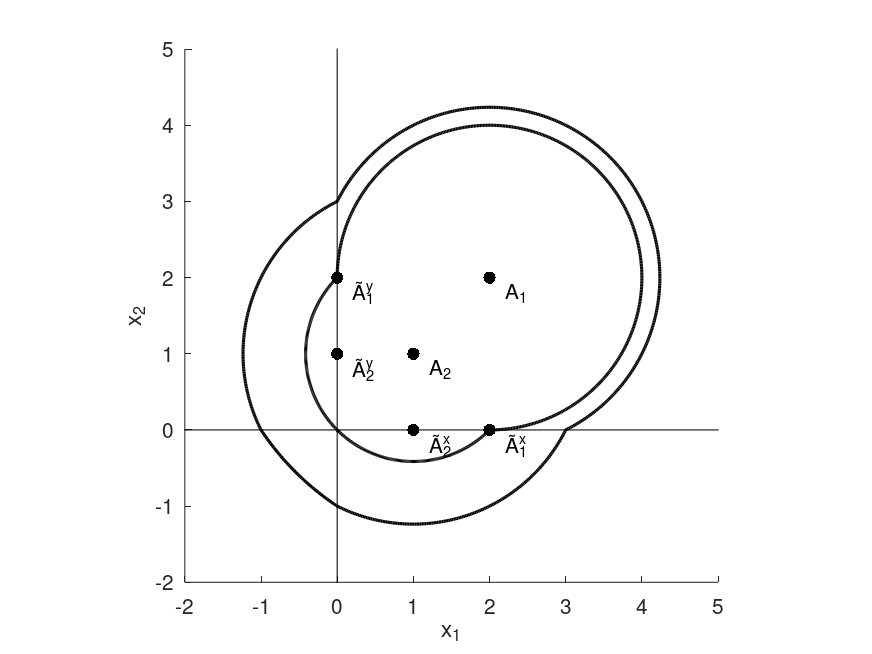
\includegraphics[width=10cm]{circ_mid}\\
\caption{\label{circ_mid}Sistema formado por (\ref{A1}) e (\ref{A2}), com $\omega=2$, $a=-1$, $c=-d=2$ e $\alpha=1/2$.}
\end{figure}

Para $\alpha<1/2$, porém, pela primeira equação de (\ref{equipott2}), $x_1(y_{min}^2)<0$, o que implica órbitas fechadas somente de segundo tipo, como pode ser visto na Fig.~\ref{circ_bef}.

\begin{figure}[H]
\centering
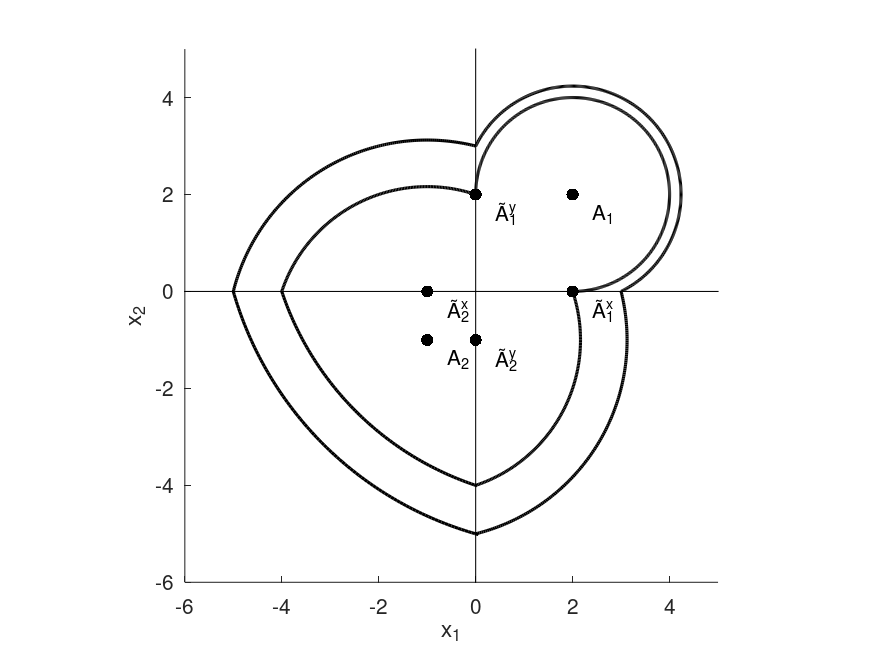
\includegraphics[width=10cm]{circ_bef}\\
\caption{\label{circ_bef}Sistema formado por (\ref{A1}) e (\ref{A2}), com $\omega=2$, $a=-1$, $c=-d=2$ e $\alpha=-1/2$.}
\end{figure}

Para $1>\alpha>1/2$, a menor órbita cruza o eixo $y$ antes de cruzar o eixo $x$, isto é, pela primeira equação de (\ref{equipott1}), $y_2(y_{min}^2)>0$. Além disso, para $y_1>y_{lim}^{1-2}$, as órbitas se encontram no regime do tipo 2, ou seja, as órbitas cruzam o eixo $x$ primeiro, o que implica um contínuo órbitas fechadas de primeiro tipo para $y_{min}^1\leq y_1<y_{lim}^{1-2}$, uma órbita do tipo limítrofe para $y_1=y_{lim}^{1-2}$, e um contínuo de órbitas de segundo tipo para $y_1>y_{lim}^{1-2}$,
como pode ser visto na Fig.~\ref{circ_aft}.

\begin{figure}[H]
\centering
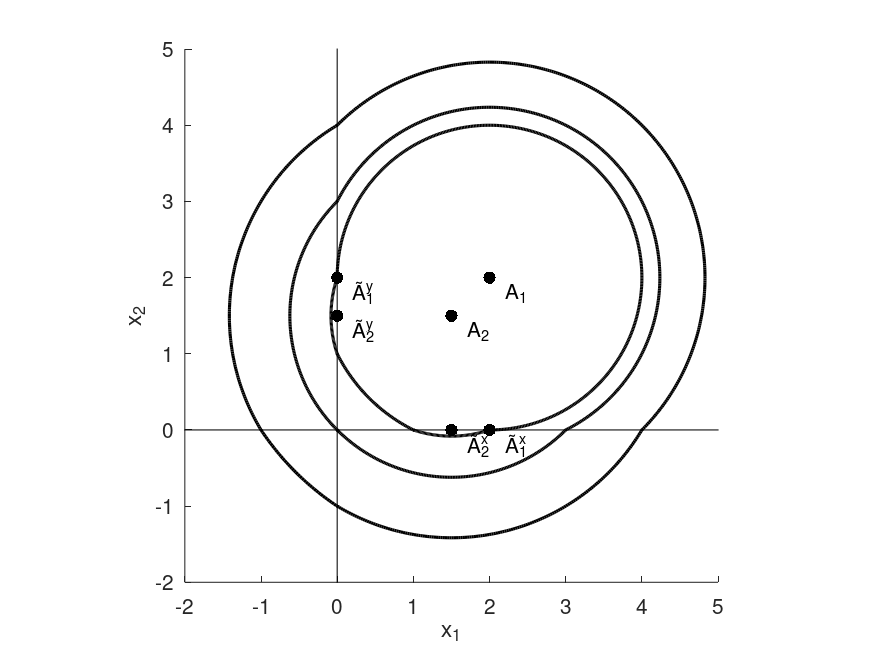
\includegraphics[width=10cm]{circ_aft}\\
\caption{\label{circ_aft}Sistema formado por (\ref{A1}) e (\ref{A2}), com $\omega=2$, $a=-1$, $c=-d=2$ e $\alpha=3/4$.}
\end{figure}

Para $\alpha\geq1$, a argumentação é semelhante ao caso anterior, porém a menor órbita é ao invés delimitada por $y_{min}^{1*}$. Logo, há um contínuo órbitas fechadas de primeiro tipo para $y_{min}^{1,*}\leq y_1<y_{lim}^{1-2}$, uma órbita do tipo limítrofe  para $y_1=y_{lim}^{1-2}$, e um contínuo de órbitas de segundo tipo para $y_1>y_{lim}^{1-2}$,
como pode ser visto na Fig.~\ref{circ_aft_inv}.

\begin{figure}[H]
\centering
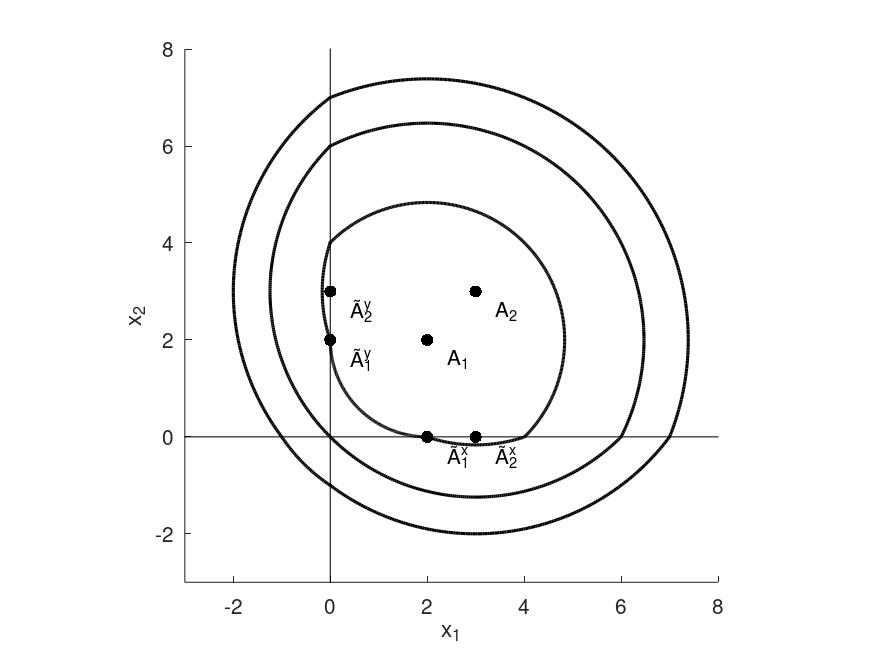
\includegraphics[width=10cm]{images/circ_aft_inv.png}\\
\caption{\label{circ_aft_inv}Sistema formado por (\ref{A1}) e (\ref{A2}), com $\omega=2$, $a=-1$, $c=-d=2$ e $\alpha=3/2$.}
\end{figure}
\end{proof}

Considere o seguinte sistema que possui em $R^{1,3}_{LV}$ o centro diferencial linear
\begin{equation}
\label{A1def}
\dot{X}=\left(\begin{array}{cc}
0 & -\frac{1}{a} \\
a & 0
\end{array}\right)\left(\begin{array}{l}
x \\
y
\end{array}\right)+\beta\left(\begin{array}{l}
\frac{1}{a} \\
-a
\end{array}\right),
\end{equation}
que possui, de (\ref{integral_cruz}), primeira integral na forma
$$H_1(x, y) = a^2 x^2 +2\beta(a^2x+y) +y^2,
$$
e que possui em $R^{2,4}_{LV}$ o centro diferencial linear 
\begin{equation}
\label{A2norm}
\dot{X}=\left(\begin{array}{cc}
0 & 1 \\
-1 & 0
\end{array}\right)\left(\begin{array}{l}
x \\
y
\end{array}\right)+\alpha\left(\begin{array}{l}
-1 \\
1
\end{array}\right),
\end{equation}
que possui, de (\ref{integral_cruz}), primeira integral na forma
$$H_2(x, y) = x^2 -2\alpha(x+y) +y^2.
$$

De forma análoga a (\ref{equipott2}), uma órbita fechada de segundo tipo obedece 
\begin{gather}
\begin{aligned}
\label{equipott2redux}
      x_1^2 -2\alpha (x_1- y_1 )- y_1^2&=0,\\
y_2^2-2\beta(y_2-a^2x_1)- a^2 x_1^2 &=0, \\
x_2^2 -2 \alpha(  x_2-y_2)- y_2^2&=0,\\
y_1^2-2\beta(y_1-a^2x_2)- a^2 x_2^2 &=0.
\end{aligned}
\end{gather}

De forma análoga a (\ref{equipott1}), uma órbita fechada de primeiro tipo obedece
\begin{gather}
\begin{aligned}
\label{equipott1redux}
(y_2 - y_1)((y_2 + y_1)-2\alpha)&=0,
\\  y_2^2-2\beta(y_2-a^2x_1) - a^2 x_1^2&=0,
\\ ( x_2- x_1) (2\alpha -(x_2+x_1)) & =0,
\\y_1^2-2\beta(y_1-a^2x_2)- a^2 x_2^2 &=0,
\end{aligned}
\end{gather}

De forma análoga aos dois casos anteriores, uma órbita fechada de terceiro tipo obedece
\begin{gather}
\begin{aligned}
\label{equipott3redux}
(y_2 - y_1)((y_2 + y_1)-2\alpha)&=0,
\\ (y_1 - y_2)((y_1 + y_2)-2\beta)&=0.
\end{aligned}
\end{gather}

\begin{lema}
\label{subs}
Uma substituição do tipo
$$
(x,y)\longrightarrow(y,x)
$$
torna o sistema formado por (\ref{A1def}) e (\ref{A2norm}) análogo a outro sistema do mesmo tipo com $a'=\frac{1}{a}$. 
\end{lema}

Sem perda de generalidade, será tomado $\beta\geq 0$, isto é, a singularidade do sistema em $R^{1,3}_{LV}$ está no primeiro quadrante. Também será só tratado o caso com $0>a>-1$, devido à substituição do Lema~\ref{subs} fornecer os valores restantes de $a<0$.

Vale notar alguns valores de $y_1$ significativos para esse sistema. Para $\alpha\leq\frac{\beta}{2}$, 
$$
y_{min}^2 = 2\alpha -\frac{2 a^2 \beta - \sqrt{4 a^4 \beta^2 + 4 a^2 (4 \alpha^2 - 8 \alpha \beta + 3 \beta^2)}}{2 a^2}
$$
define a menor órbita de tipo 2 do sistema, que passa e é limitada pelo ponto $\tilde{A}_1^x$.

Para $\alpha\geq\frac{\beta}{2}$,  
\begin{equation}
\label{y_lim_1-2}
y_{lim}^{1-2}=2\alpha
\end{equation}
define a órbita limítrofe tipo 1-2, que passa pela origem, isto é, $y_{lim}^{1-2}=y_2(0)^{-1}$ com a nomenclatura para órbitas do tipo 1, e $y_{lim}^{1-2}=x_1(0)^{-1}$ com a nomenclatura para órbitas do tipo 2.

Para $\beta>\alpha\geq\frac{\beta}{2}$, 
$$
y_{min}^1=2\alpha-\beta + \sqrt{\beta^2 + a^2 (4 \alpha^2 - 8 \alpha \beta + 3 \beta^2)}
$$
define a menor órbita do tipo 1, que passa e é limitada pelo ponto $\tilde{A}^x_1$. Em particular, quando $\alpha=\frac{\beta}{2}$, essa órbita também é limítrofe tipo 1-2. 

Para $\alpha\geq\beta$,
$$y_{lim}^{3-1}=2\alpha-\beta+\sqrt{-\beta^2(a^2-1)}$$
define a órbita limítrofe tipo 3-1, que passa e é limitada pelo ponto $\tilde{A}^x_1$.
\begin{proposition}
\label{propredux}
Dado um sistema formado por (\ref{A1def}) e (\ref{A2norm}), as seguintes afirmações são verdadeiras.
\begin{enumerate}[(a)]
\item Se $\alpha=\beta$, existe um contínuo de órbitas fechadas de terceiro tipo para $ y_{min}^3\leq y_1<y_{lim}^{3-1}$, com uma órbita limítrofe fechada para $y_1=y_{lim}^{3-1}$, de primeiro tipo para $y_{lim}^{3-1}< y_1<y_{lim}^{1-2}$, com uma órbita limítrofe fechada para $y_1=y_{lim}^{1-2}$, e nenhuma órbita fechada para $y_1>y_{lim}^{1-2}$;
\item Se $\alpha>\beta$, não existem órbitas fechadas;
\item Se $\frac{\beta}{2}\leq\alpha<\beta$, existe uma órbita fechada, que é de segundo tipo;
\item Se $\leq\alpha<\frac{\beta}{2}$, existe uma órbita fechada, que é de segundo tipo;
\item Se $\alpha<$, não existem órbitas fechadas.
\end{enumerate}
\end{proposition}
\begin{proof}
Começando pelo item (a), para $\alpha=\beta$, analisando a órbita limítrofe tipo 1-2 com $y_1=y_{lim}^{1-2}$ tem-se que, tanto por (\ref{equipott1redux}) quanto por (\ref{equipott2redux}), é direto conferir que ela é fechada. 

Para $y_{lim}^{3-1}<y_1<y_{lim}^{1-2}$ as órbitas são de tipo 1, e de (\ref{equipott1redux}), é direto obter que $y_2=2\alpha-y_1$, 
\begin{align*}
x_1&=\beta-\frac{\sqrt{ a^2( a^2\beta^2 +  y_2 (y_2 - 2 \beta))}}{ a^2}\\&=\alpha-\frac{\sqrt{ a^2(a^2 \alpha^2 +  y_1 (y_1 - 2 \alpha))}}{ a^2}
\end{align*}
e, de $x_2=2\alpha-x_1$,  
$$
x_2=\alpha+\frac{\sqrt{ a^2(a^2 \alpha^2 +  y_1 (y_1 - 2 \alpha))}}{ a^2}.
$$
Por outro lado, da quarta equação de (\ref{equipott1redux}), tem-se que
\begin{align*}
x_2^*&=\beta+\frac{\sqrt{ a^2(a^2 \beta^2 +  y_1 (y_1 - 2 \beta))}}{ a^2}\\
&=\alpha+\frac{\sqrt{ a^2(a^2 \alpha^2 +  y_1 (y_1 - 2 \alpha))}}{ a^2},
\end{align*}
que coincide com a expressão obtida das 3 primeiras equações, logo a órbita é fechada. 

Já para $y_{min}^3\leq y_1<y_{lim}^{3-1}$ as órbitas são de tipo 3, e de (\ref{equipott3redux}) tem-se que $y_2=2\alpha-y_1$ e $y_3=2\beta-y_2$, logo $y_3=y_1$, isto é, a órbita é fechada. Em particular, a órbita limítrofe tipo 3-1 com $y_1=y_{lim}^{3-1}$ também é fechada, uma vez que, de (\ref{equipott3redux}) e (\ref{equipott1redux}),
$$
\lim_{y_1\to (y_{lim}^{3-1})^+}y_3=\lim_{y_1\to (y_{lim}^{3-1})^-}y_3=y_1.
$$

Para $y_1>y_{lim}^{1-2}$ as órbitas são de tipo 2, e de (\ref{equipott1redux}), é direto obter que $x_1=2\alpha-y_1$, 
\begin{align*}
y_2&=\beta-\sqrt{ a^2x_1 (x_1 - 2 \beta)+\beta^2}\\&=\alpha-\sqrt{ a^2y_1 (y_1 - 2 \alpha)+\alpha^2}
\end{align*}
e, de $x_2=2\alpha-y_2$,  
$$
x_2=\alpha+\sqrt{ a^2y_1 (y_1 - 2 \alpha)+\alpha^2}
$$
logo 
\begin{align*}
y_3&=\beta+\sqrt{ a^4y_1 (y_1 - 2 \beta)+\beta^2}
\\&=\alpha+\sqrt{ a^4y_1 (y_1 - 2 \alpha)+\alpha^2}
\end{align*}
e, derivando com respeito a $y_1$
$$y_3'=\frac{a^4(y_1-\alpha)}{\sqrt{ a^4y_1 (y_1 - 2 \alpha)+\alpha^2}},$$
que é monótona crescente e possui 

$$\lim_{y_1\to \infty}y_3'=a^2<1.$$

Além disso, 
$$\lim_{y_1\to (y_{lim}^{1-2})^+} y_3'=a^4<a^2,$$
logo $y_3<y_1$ para $y_1>y_{lim}^{1-2}$, então não existem órbitas fechadas (de segundo tipo) nesse intervalo. Em particular, a órbita limítrofe tipo 1-2 com $y_1=y_{lim}^{3-1}$ também é fechada, uma vez que, de (\ref{equipott2redux}) e (\ref{equipott1redux}),
$$
\lim_{y_1\to (y_{lim}^{1-2})^+}y_3=\lim_{y_1\to (y_{lim}^{1-2})^-}y_3=y_1,
$$
completando a prova da Proposição~\ref{propredux} (a), que é ilustrada na Fig.~\ref{2x1_yeqx_eq}.

\begin{figure}[H]
\centering
\begin{table}[H]
\centering
\begin{tabular}{cc}
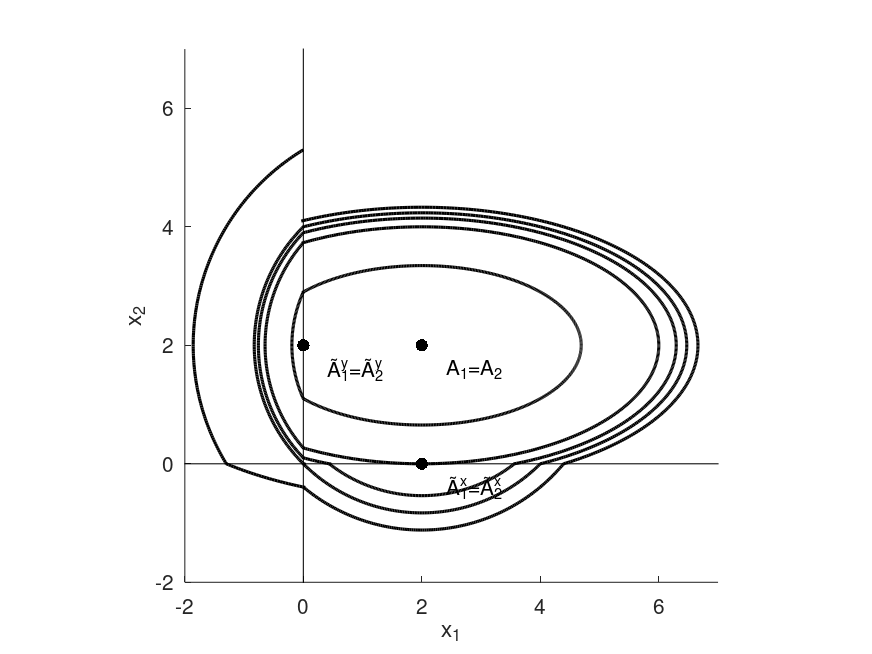
\includegraphics[width=7cm]{images/2x1_yeqx_eq.png}
&
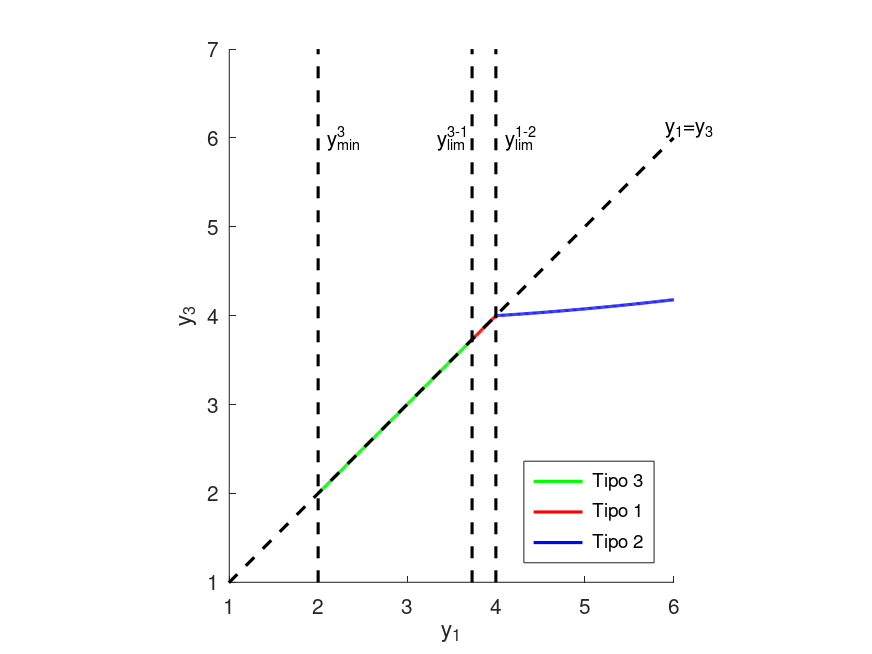
\includegraphics[width=7cm]{images/2x1_yeqx_eq_y3.png}
\end{tabular}
\end{table}
\caption{\centering\label{2x1_yeqx_eq}Sistema formado por (\ref{A1def}) e (\ref{A2norm}) na esquerda e seu respectivo gráfico da diferença $y_3(y_1)$ na direita, com $a=-\frac{1}{2}$ e $\alpha=\beta=2$.}
\end{figure}

Já no caso (b), para $y_{min}^3\leq y_1<y_{lim}^{3-1}$, as órbitas são de tipo 3, e de (\ref{equipott3redux}) tem-se que $y_2=2\alpha-y_1$ e $y_3=2\beta-y_2$, logo $y_3=y_1+2(\beta-\alpha)<y_1$ para todo o intervalo, pois $\alpha>\beta$.

Para $y_{lim}^{3-1}< y_1<y_{lim}^{1-2}$ as órbitas são de tipo 1, e de forma análoga ao cálculo para $\alpha=\beta$ obtém-se que, de (\ref{equipott1redux}),
$$
x_2=
2\alpha-\beta+\frac{\sqrt{ a^2( a^2\beta^2 +  (2\alpha-y_1) (2(\alpha-\beta)-y_1))}}{ a^2}
$$
e
\begin{gather}
\begin{aligned}
\label{r_1}
r_1(y_1)&=x_2-x_2^*
\\&=
2(\alpha-\beta)+\frac{\sqrt{ a^2( a^2\beta^2 +  (2\alpha-y_1) (2(\alpha-\beta)-y_1))}-\sqrt{ a^2(a^2 \beta^2 +  y_1 (y_1 - 2 \beta))}}{ a^2}.\nonumber
\end{aligned}
\end{gather}

Note que uma órbita fechada ocorre quando $r_1(y_1)=0$. Analisando o extremo do intervalo tem-se que
\begin{equation}
\label{r_1-2}
    \lim_{y_1\rightarrow (y_{lim}^{1-2})^-}r_1(y_1)=2\alpha-\beta-\frac{\sqrt{ a^2(a^2 \beta^2 +  4\alpha (\alpha - \beta))}}{ a^2}<0,
    \end{equation}
uma vez que, de $|a|<1$,
$$
a^2(2\alpha-\beta)^2=a^2\beta^2+4a^2\alpha(\alpha-\beta)<a^2 \beta^2 +  4\alpha (\alpha - \beta),
$$
e usando o fato de que $2\alpha-\beta>0\Rightarrow\sqrt{(2\alpha-\beta)^2}=2\alpha-\beta$.

Além disso
\begin{equation}
\label{r_3-1}
\lim_{y_1\to (y_{lim}^{3-1})^+}r_1(y_1)=2\left(\alpha-\beta-\frac{\sqrt{a^{2}(\alpha-\beta)\left(\alpha-\beta+\sqrt{\left(1-a^{2}\right) \beta^{2}}\right)}}{a^{2}}\right)<0,
\end{equation}
uma vez que, analogamente,
$$
a^2(\alpha-\beta)^2<(\alpha-\beta)\left(\alpha-\beta+\sqrt{\left(1-a^{2}\right) \beta^{2}}\right).
$$

Derivando com respeito a $y_1$,
$$
r_1'(y_1)=\frac{\beta-y_1}{\sqrt{a^2 (y_1^2 - 2 y_1 \beta + a^2 \beta^2)}} + \frac{y_1 - 2 \alpha + \beta}{\sqrt{a^2 (y_1^2 - 4 y_1 \alpha + 4 \alpha^2 + 2 y_1 \beta - 4 \alpha \beta + a^2 \beta^2)}}.
$$

Tem-se que
\begin{align*}
(y_1 - 2 \alpha + \beta)^2&=4\alpha^2  + \beta(\beta+2 y_1) + y_1^2 - 4 \alpha (y_1+\beta)
\\&>a^2 (4 \alpha^2 +\beta(a^2\beta+2y_1)+y_1^2 - 4 \alpha (y_1  +\beta ))
\\&=a^2 (y_1^2 - 4 y_1 \alpha + 4 \alpha^2 + 2 y_1 \beta - 4 \alpha \beta + a^2 \beta^2),
\end{align*}
que vale para as raízes dos dois lados da equação, visto que $y_1 - 2 \alpha + \beta>0$ e $a^2 (y_1^2 - 4 y_1 \alpha + 4 \alpha^2 + 2 y_1 \beta - 4 \alpha \beta + a^2 \beta^2)>0$ para $y_1\geq y_{lim}^{3-1}$. Além disso
\begin{gather}
\begin{aligned}
\label{ineq1}
(\beta-y_1)^2&=y_1^2-2y_1\beta+\beta^2
\\&>a^2 (y_1^2 - 2 y_1 \beta + a^2 \beta^2),
\end{aligned}    
\end{gather}
logo, como $\beta-y_1<0$, $a^2 (y_1^2 - 2 y_1 \beta + a^2 \beta^2)>0$ para $y_1\geq y_{lim}^{3-1}$ e pelo acima
$$
\frac{\beta-y_1}{y_1 - 2 \alpha + \beta}< -\frac{\sqrt{a^2 (y_1^2 - 2 y_1 \beta + a^2 \beta^2)}}{y_1 - 2 \alpha + \beta}<-\frac{\sqrt{a^2 (y_1^2 - 2 y_1 \beta + a^2 \beta^2)}}{\sqrt{a^2 (y_1^2 - 4 y_1 \alpha + 4 \alpha^2 + 2 y_1 \beta - 4 \alpha \beta + a^2 \beta^2)}}.
$$
Portanto
$$
r_1'(y_1)>0,\quad y_{lim}^{3-1}< y_1<y_{lim}^{1-2},
$$
e por (\ref{r_3-1}) e (\ref{r_1-2}) não existem órbitas fechadas de primeiro tipo.

Para $y_1>y_{lim}^{1-2}$ as órbitas são de tipo 2, e de forma análoga ao cálculo para $\alpha=\beta$ obtém-se que, de (\ref{equipott2redux}),
$$
x_2=2 \alpha-\beta+\sqrt{ a^2(2\alpha-y_1) (2(\alpha-\beta)-y_1)+\beta^2}
$$
e
\begin{gather}
\begin{aligned}
\label{r_2}
r_2(y_1)&=x_2-x_2^*
\\&=
2(\alpha-\beta)+\sqrt{ a^2(2\alpha-y_1) (2(\alpha-\beta)-y_1)+\beta^2}-\frac{\sqrt{ a^2(a^2 \beta^2 +  y_1 (y_1 - 2 \beta))}}{ a^2}.\nonumber
\end{aligned}
\end{gather}

Novamente uma órbita fechada ocorre quando $r_2(y_1)=0$. Analisando o extremo do intervalo tem-se que
\begin{equation}
\label{r_2_1-2}
    \lim_{y_1\rightarrow (y_{lim}^{1-2})^-}r_2(y_1)=2\alpha-\beta-\frac{\sqrt{ a^2(a^2 \beta^2 +  4\alpha (\alpha - \beta))}}{ a^2}=\lim_{y_1\rightarrow (y_{lim}^{1-2})^-}r_1(y_1)<0.
    \end{equation}

Além disso
\begin{equation}
\label{r_infty}
\lim_{y_1\to \infty}r_2(y_1)=-\infty<0.
\end{equation}

Derivando com respeito a $y_1$,
$$
r_2'(y_1)=\frac{\beta-y_1}{\sqrt{a^2 (y_1^2 - 2 y_1 \beta + a^2 \beta^2)}} + \frac{a^2(y_1 - 2 \alpha + \beta)}{\sqrt{ a^2(2\alpha-y_1) (2(\alpha-\beta)-y_1)+\beta^2}}.
$$
Note que
\begin{align*}
a^4(y_1 - 2 \alpha + \beta)^2&=a^4(4\alpha^2  +2 \beta y_1 + y_1^2 - 4 \alpha (y_1+\beta))+a^4\beta^2
\\&<a^2(4\alpha^2+2\beta y_1+y_1^2-4\alpha(y_1+\beta))+\beta^2
\\&= a^2(2\alpha-y_1) (2(\alpha-\beta)-y_1)+\beta^2.
\end{align*}

Por (\ref{ineq1}) e como ainda $\beta-y_1<0$, $a^2 (y_1^2 - 2 y_1 \beta + a^2 \beta^2)>0$, $a^2(y_1 - 2 \alpha + \beta)>0$ e $a^2(2\alpha-y_1) (2(\alpha-\beta)-y_1)+\beta^2>0$ para $y_1> y_{lim}^{1-2}$, tem-se que
$$
-\frac{\beta-y_1}{a^2(y_1 - 2 \alpha + \beta)}> \frac{\sqrt{a^2 (y_1^2 - 2 y_1 \beta + a^2 \beta^2)}}{a^2(y_1 - 2 \alpha + \beta)}>\frac{\sqrt{a^2 (y_1^2 - 2 y_1 \beta + a^2 \beta^2)}}{\sqrt{a^2(2\alpha-y_1) (2(\alpha-\beta)-y_1)+\beta^2}}.
$$
Portanto
\begin{equation}
\label{r_2'}
r_2'(y_1)<0,\quad y_1> y_{lim}^{1-2},
\end{equation}
e por (\ref{r_infty}) e (\ref{r_2_1-2}) não existem órbitas fechadas de segundo tipo. 

Para $y_1=y_{lim}^{1-2}$, como, de (\ref{r_2_1-2}), os limites laterais de $r_1$ e $r_2$ coincidem e são menores que 0, não há órbita fechada também, completando a prova da Proposição~\ref{propredux} (b), que é ilustrada na Fig.~\ref{prepb}.

\begin{figure}[H]
\centering
\begin{table}[H]
\centering
\begin{tabular}{cc}
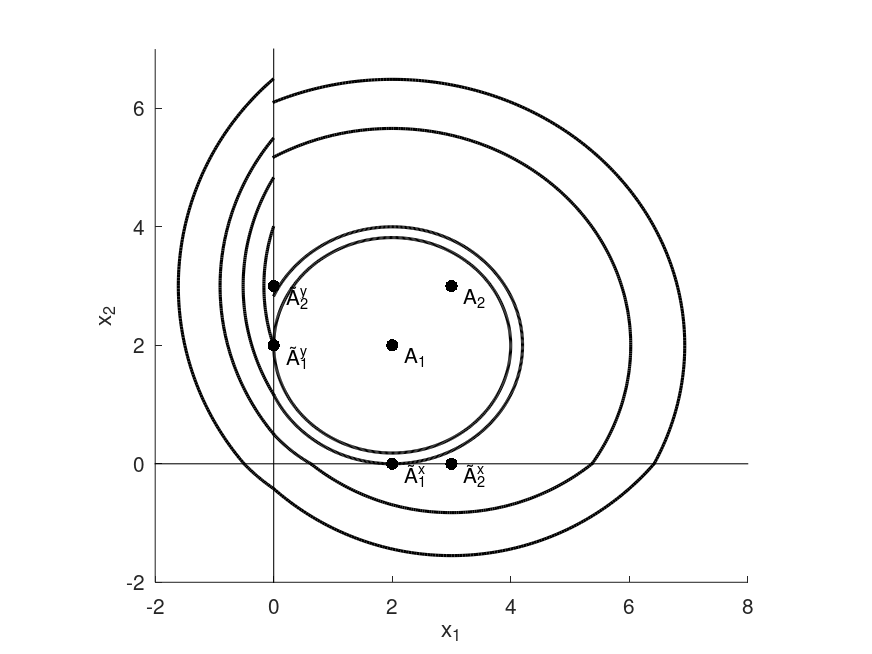
\includegraphics[width=7cm]{images/1.1x1_yeqx_zzaft.png}
&
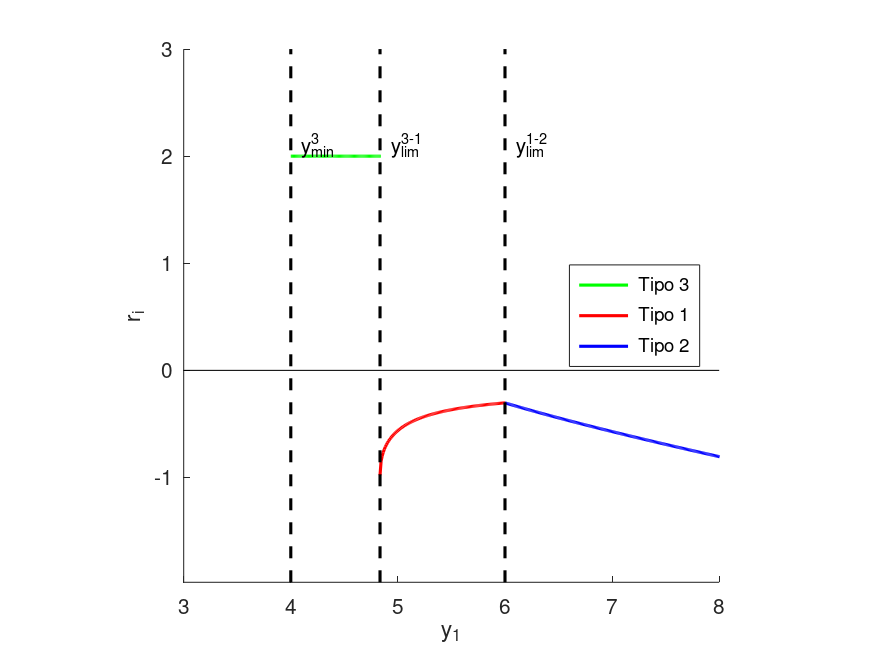
\includegraphics[width=7cm]{images/1.1x1_yeqx_zzaft_diff.png}
\end{tabular}
\end{table}
\caption{\centering\label{prepb}Sistema formado por (\ref{A1def}) e (\ref{A2norm}) na esquerda e seu respectivo gráfico da diferença $r_i(y_1),\  i=1,2,3$ na direita, com $a=-\frac{10}{11}$, $\alpha=3$ e $\beta=2$.}
\end{figure}

Analisando o caso (c), para $y_{min}^1\leq y_1<y_{lim}^{1-2}$ as órbitas são de tipo 1. Definindo
\begin{equation}
\label{y_min_inverse}
y_{min}^{1*}=\beta+\sqrt{\beta^2(1-a^2)},
\end{equation}
note que esse valor define a menor órbita no sentido inverso do sistema, como pode ser visto na Fig.~\ref{y_min_lim}, e
$$
x_2^*\left(y_{min}^{1*}\right)=\beta
$$
logo, para $y_1<y_{min}^{1*}$, pela restrição de que $x_2>\beta$, $x_2^*(y_1)$ não está bem definido (mesmo que $x_2(y_1)$ esteja para $y_{lim}^1\leq y_1<y_{min}^{1*}$, no sentido usual). Isso implica que, para $y_{min}^1\leq y_1<y_{min}^{1*}$, $y_3(y_1)\geq y_{min}^{1*}>y_1$, logo não há órbitas fechadas.

\begin{figure}[H]
\centering
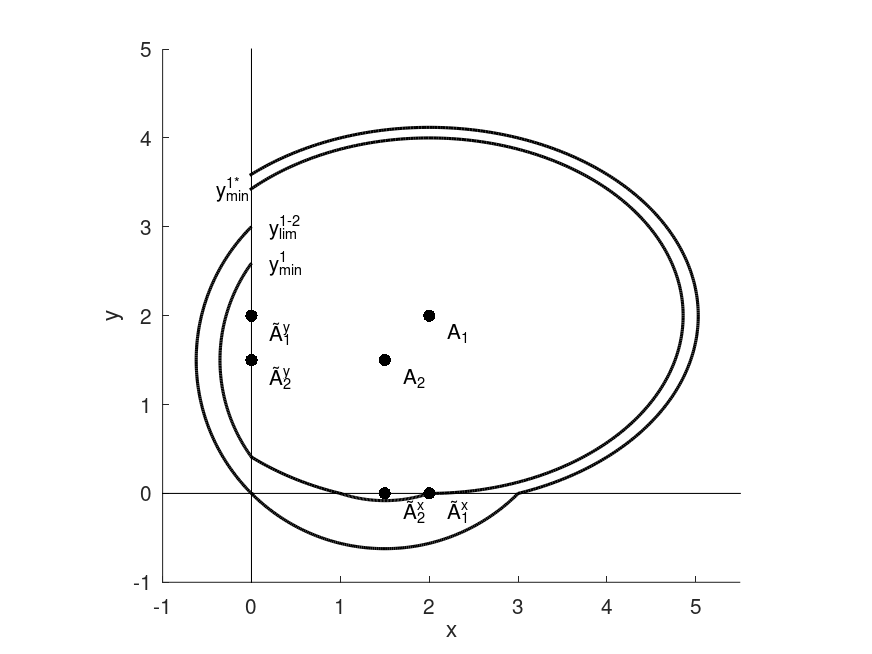
\includegraphics[width=10cm]{images/y_min_lim.png}\\
\caption{\label{y_min_lim}Sistema formado por (\ref{A1def}) e (\ref{A2norm}), com $a=-0.7$, $\alpha=\frac{3}{2}$ e $\beta=2$.}
\end{figure}

Analisando primeiramente o caso no qual $y_{min}^{1*}\geq y_{lim}^{1-2}$, isto é, a menor órbita no sentido inverso já começa em uma região na qual, no sentido usual, as órbitas são de segundo tipo, como pode ser visto na Fig.~\ref{y_min_lim}; para $y_{min}^{1*} > y_1\geq y_{min}^1$, como visto acima, não existem órbitas fechadas.  

Para $y_1\geq y_{min}^{1*}\geq y_{lim}^{1-2}$ as órbitas são de tipo 2. Analisando o extremo do intervalo tem-se que
\begin{equation}
\label{r_2_min_inv}
    \lim_{y_1\rightarrow (y_{min}^{1*})^-}r_2(y_1)=2(\alpha-\beta)+\sqrt{\beta^2(1-a^4)+4a^2(\beta-\alpha)\left(\beta\left(1+\sqrt{1-a^2}\right)-\alpha\right)}>0,
\end{equation}
uma vez que, como $-\alpha<-\frac{\beta}{2}$,
\begin{align*}
4(\alpha-\beta)^2&=4((1-a^2)+a^2)(\beta-\alpha)(\beta-\alpha)
\\&<\beta^2(1-a^2)+4a^2(\beta-\alpha)\left(\beta\left(1+\sqrt{1-a^2}\right)-\alpha\right)
\\&=\beta^2(1-a^4)+4a^2(\beta-\alpha)\left(\beta\left(1+\sqrt{1-a^2}\right)-\alpha\right)
\end{align*}
e usando o fato de que $\alpha-\beta<0$ e $\beta^2(1-a^4)+4a^2(\beta-\alpha)\left(\beta\left(1+\sqrt{1-a^2}\right)-\alpha\right)>0$.

Além disso, vale (\ref{r_infty}). A análise da derivada $r_2'(y_1)$ é idêntica e obtém-se (\ref{r_2'}). Logo, somado à (\ref{r_2_min_inv}), é demonstrado que existe um ciclo limite (de segundo tipo) para $y_1> y_{min}^{1*}$.

Já no caso $y_{min}^{1*}< y_{lim}^{1-2}$, para $y_{min}^{1*} > y_1\geq y_{min}^1$, novamente, não existem órbitas fechadas.  

Para $y_{lim}^{1-2}>y_1\geq y_{min}^{1*}$, tem-se que, de (\ref{r_1}),
\begin{equation}
    \label{r_1_y_inv}
    r_1(y_{min}^{1*})=2(\alpha-\beta)+2\sqrt{a^2(\beta-\alpha)\left(\beta\left(1+\sqrt{1-a^2}\right)-\alpha\right)}>0,
\end{equation}
uma vez que, de $|a|<1$,
\begin{align*}
a^2(\alpha-\beta)^2&=a^2(\beta-\alpha)(\beta-\alpha)
\\&<(\beta-\alpha)\left(\beta\left(1+\sqrt{1-a^2}\right)-\alpha\right),
\end{align*}
e usando o fato de que $\alpha-\beta<0$ e $a^2(\beta-\alpha)\left(\beta\left(1+\sqrt{1-a^2}\right)-\alpha\right)>0$, segue (\ref{r_1_y_inv}).

Para $y_1>y_{lim}^{1-2}$ as órbitas são de tipo 2. Primeiramente será tratado o caso com $y_{min}^{1*}<y_{lim}^{1-2}$, no qual $r_2(y_1)$ é também obtido como (\ref{r_2}). Analisando o extremo do intervalo tem-se que
\begin{equation}
\label{r_2_1-2-c}
    \lim_{y_1\rightarrow (y_{lim}^{1-2})^-}r_2(y_1)=2\alpha-\beta-\frac{\sqrt{ a^2(a^2 \beta^2 +  4\alpha (\alpha - \beta))}}{ a^2}=\lim_{y_1\rightarrow (y_{lim}^{1-2})^-}r_1(y_1)>0,
    \end{equation}
uma vez que, de $|a|<1$ e $\alpha<\beta$,
$$
a^2(2\alpha-\beta)^2=a^2\beta^2+4a^2\alpha(\alpha-\beta)>a^2 \beta^2 +  4\alpha (\alpha - \beta),
$$
e usando o fato de que $2\alpha-\beta>0$ e $a^2\beta^2+4a^2\alpha(\alpha-\beta)>a^2 \beta^2 +  4\alpha (\alpha - \beta)>0$.

Novamente, vale (\ref{r_infty}),  (\ref{r_2'}) e, somado à (\ref{r_2_1-2-c}), é demonstrado que existe um ciclo limite (de segundo tipo) para $y_1>y_{lim}^{1-2}$ com $y_{min}^{1*}<y_{lim}^{1-2}$, completando a prova da Proposição~\ref{propredux} (c), que é ilustrada na Fig.~\ref{prepc} e Fig.~\ref{prepc2}.

\begin{figure}[H]
\centering
\begin{table}[H]
\centering
\begin{tabular}{cc}
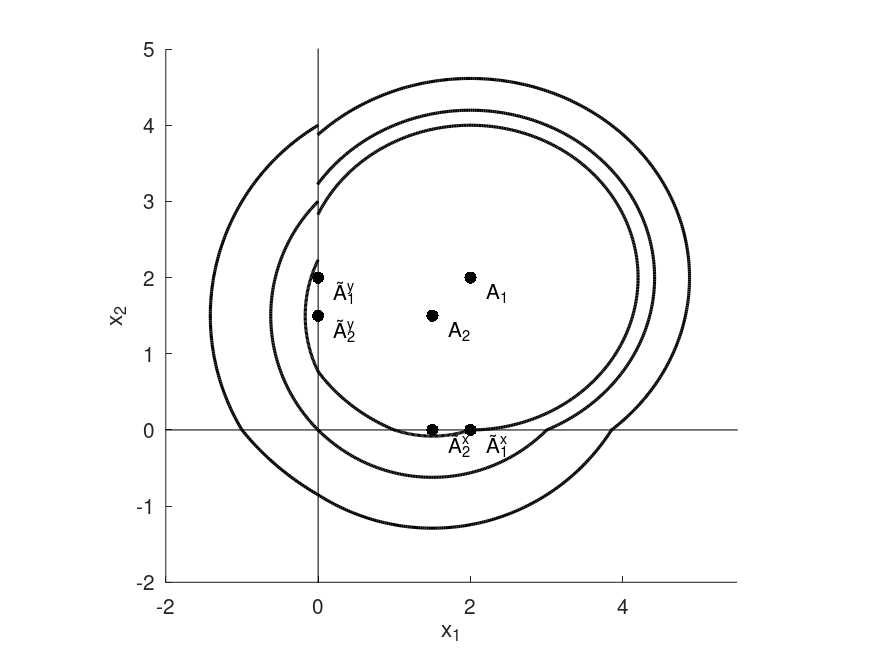
\includegraphics[width=7cm]{images/1.1x1_yeqx_zaft.png}
&
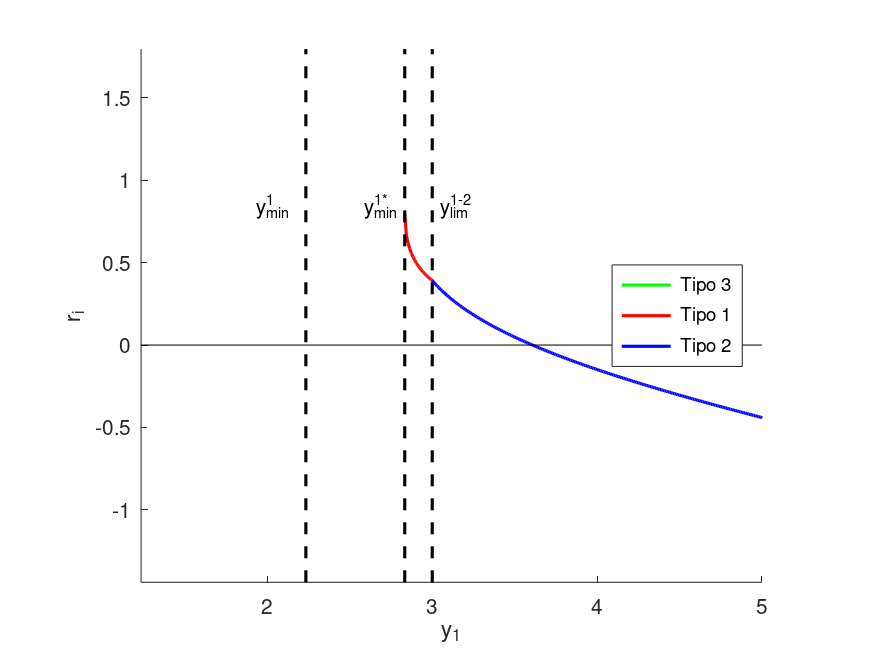
\includegraphics[width=7cm]{images/1.1x1_yeqx_zaft_diff.png}
\end{tabular}
\end{table}
\caption{\centering\label{prepc}Sistema formado por (\ref{A1def}) e (\ref{A2norm}) na esquerda e seu respectivo gráfico da diferença $r_i(y_1),\  i=1,2,3$ na direita, com $a=-\frac{10}{11}$, $\alpha=\frac{3}{2}$ e $\beta=2$. Note que $y_{min}^{1*}< y_{lim}^{1-2}$.}
\end{figure}

\begin{figure}[H]
\centering
\begin{table}[H]
\centering
\begin{tabular}{cc}
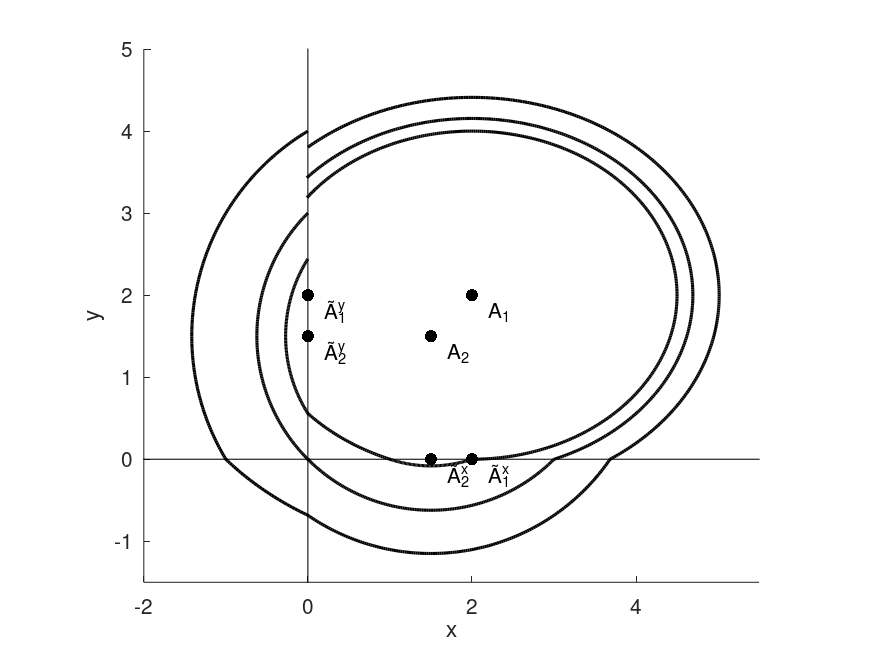
\includegraphics[width=7cm]{images/1.1x1_yeqx_zaft_2.png}
&
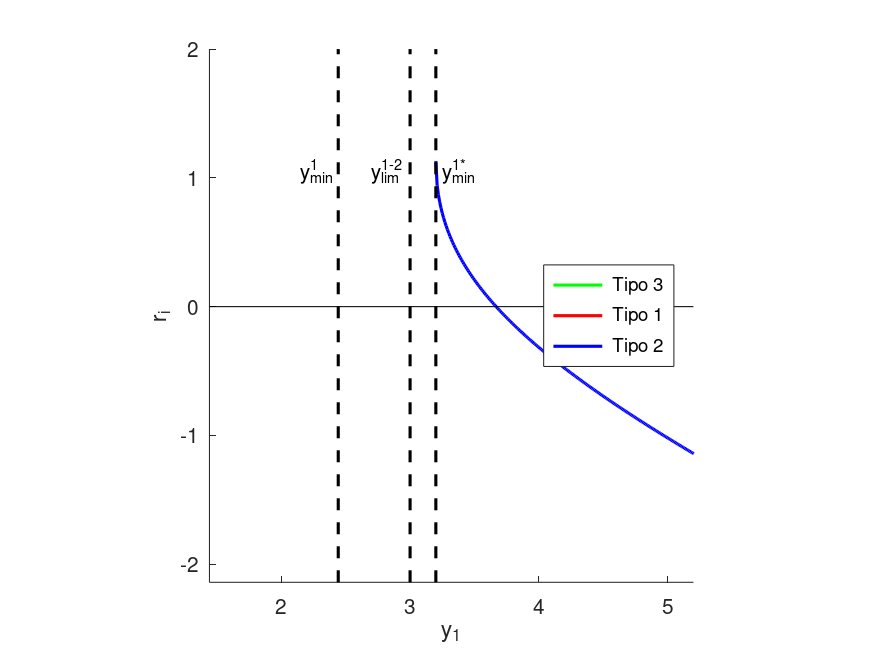
\includegraphics[width=7cm]{images/1.1x1_yeqx_zaft_diff_2.png}
\end{tabular}
\end{table}
\caption{\centering\label{prepc2}Sistema formado por (\ref{A1def}) e (\ref{A2norm}) na esquerda e seu respectivo gráfico da diferença $r_i(y_1),\  i=1,2,3$ na direita, com $a=-\frac{4}{5}$, $\alpha=\frac{3}{2}$ e $\beta=2$. Note que $y_{min}^{1*}> y_{lim}^{1-2}$.}
\end{figure}

Para o caso (d) e (e), basta analisar $y_1\geq max(y_{min}^2,)$. Ainda vale (\ref{r_2'}) e (\ref{r_infty}), portanto
\begin{gather}
\begin{aligned}
\label{r_2_2}
\lim_{y_1\rightarrow (y_{min}^2)^-}r_2(y_1)=&2 (\alpha-\beta)
-\frac{1}{a^{2}}\left[\beta\left(a^{4}(-(8 \alpha-5 \beta))-8 \alpha\right)+a^{2}\left(4 \alpha^{2}-4 \alpha \beta+\beta^{2}\right)+\right. \\&
\left.\left(4 a^{6}+3\right) \beta^{2}+2\left(\left(2 a^{2}+1\right) \beta-2 \alpha\right) \sqrt{a^{2}\left(\left(a^{2}+3\right) \beta^{2}+4 \alpha^{2}-8 \alpha \beta\right)}+4 \alpha^{2}\right]^{\frac{1}{2}}\\&
+\left[2\left(2 a^{2}-1\right) \beta \sqrt{a^{2}\left(\left(a^{2}+3\right) \beta^{2}+4 \alpha^{2}-8 \alpha \beta\right)}+4\left(\alpha^{2}-2 \alpha \beta+\beta^{2}\right)+\right.\\&\qquad \qquad \qquad \qquad\quad \qquad\qquad\qquad\qquad\qquad\qquad
\left.\left(4 a^{6}-4 a^{4}+a^{2}\right) \beta^{2}\right]^{\frac{1}{2}}.
\end{aligned}    
\end{gather}

\end{proof}

\newpage
$$
8a(1- \alpha )cx_1 + 8a (1-\alpha) c x_2= 8a(\alpha-1)dy_2+8a (\alpha-1) d y_1
$$
$$
8a(1- \alpha )cx_1 -8a \alpha c x_2	+y_1^2\omega^2= 4a^2x_2^2 + 8a(\alpha-1)dy_2+8a \alpha d y_1
$$
$$
8a[(1- \alpha )(cx_1+dy_2) -\alpha (c x_2+ d y_1)]= 4a^2x_2^2 -y_1^2\omega^2
$$
$$
8a(1- \alpha )cx_1 -8a \alpha  \frac{d^2y_1y_2}{c x_1}	+y_1^2\omega^2= \omega^2\frac{d^2y_1^2y_2^2}{c^2x_1^2} + 8a(\alpha-1)dy_2+8a \alpha d y_1
$$
$$
y_1^2\omega^2= d^2(\omega^2z^2+8a \alpha  z)+ 8a(\alpha-1)(dy_2+cx_1)+8a \alpha d y_1
$$

Se $\alpha\geq\beta$, $x_1=\pi_1\circ\tilde{A}^x_1$ (limítrofe tipo 3-1):
$$y_1=2\alpha-\beta+\sqrt{-\beta^2(a^2-1)}$$

Se $\beta>\alpha\geq\frac{\beta}{2}$, $x_2=\pi_1\circ\tilde{A}^x_1$ (menor órbita tipo 1, quando $\alpha=\frac{\beta}{2}$, essa órbita também é limítrofe tipo 1-2):
$$
y_1=2\alpha-\beta + \sqrt{\beta^2 + a^2 (4 \alpha^2 - 8 \alpha \beta + 3 \beta^2)}
$$

Se $\alpha<\frac{\beta}{2}$, $x_2=\pi_1\circ\tilde{A}^x_1$ (menor órbita tipo 2):
$$
y_1 = 2\alpha -\frac{2 a^2 \beta - \sqrt{4 a^4 \beta^2 + 4 a^2 (4 \alpha^2 - 8 \alpha \beta + 3 \beta^2)}}{2 a^2}
$$
$$
y_2=2\alpha-y_1
$$
$$
x_1=\beta-\frac{\sqrt{ a^2( a^2\beta^2 +  y_2 (y_2 - 2 \beta))}}{ a^2}
$$
$$
x_1=\beta-\frac{\sqrt{ a^2( a^2\beta^2 +  (2\alpha-y_1) (2(\alpha-\beta)-y_1 ))}}{ a^2}
$$
$$
y_3=\frac{1}{2}\left(2 \beta + \sqrt{4 \beta^2 - 4 (y_1(4 \alpha - 2 \beta)-4 (\alpha - \beta) (a^2x_2 + \alpha(1-a^2)) - y_1^2 )}\right).
$$
Além disso, 
$$\underset{y_1\rightarrow (y_{lim}^{3-1})^+}{lim}=a^4<a^2,$$

$$
a^2((y_1^2 - 2 y_1 \beta + a^2 \beta^2)-(y_1^2 - 4 y_1 \alpha + 4 \alpha^2 + 2 y_1 \beta - 4 \alpha \beta + a^2 \beta^2))=4a^2(\alpha- \beta) (y_1-\alpha)>0.
$$


%--------- Referências -------------------------------------------------
\bibliographystyle{plainnat}
\bibliography{monografia}

\end{document}
